% ~7 min
\partframe{Background}{Recursion Schemes}

\begin{frame}
  \frametitle{Functors and Algebras}
  \[ \List\,A \cong 1 + A \times \List\,A = F\,(\List\,A) \]
  \begin{itemize}
    \item \emph{Algebra}: $a : F\,B \to B$.
    \item \emph{Initial algebra}: the constructors,
      $\inn = [\op{nil}, \op{cons}]$.
  \end{itemize}
  \speakernote{Lists are the least fixed point of F X = 1 + A x X. An
    algebra says what to do with each constructor: for lists, a base case
    and a step, [base, step] : 1 + A x B -> B. The constructors themselves
    are the initial algebra. F f is fmap f: it applies f to the recursive
    position only. Go fast if the audience knows this.}
\end{frame}

\begin{frame}
  \frametitle{Catamorphisms (Folds)}
  \[
    \begin{tikzcd}[alt={Commuting square: F of mu F maps to F B by F of
        the fold; in maps F mu F to mu F; a maps F B to B; the fold maps
        mu F to B.}]
      F\,\mu F \arrow[r, "F\,\cata{a}"] \arrow[d, "\inn"'] \& F\,B
        \arrow[d, "a"] \\
      \mu F \arrow[r, "\cata{a}"', dashed] \& B
    \end{tikzcd}
    \qquad
    f = \cata{a} \iff f \circ \inn = a \circ F\,f
  \]
  A \emph{unique} arrow out of the initial algebra.
  \speakernote{The fold is the unique map making the square commute; the
    equivalence is the universal property, and every law later follows from
    this uniqueness. For lists, the fold of [base, step] is foldr step base.
    Recursion follows the structure of the data.}
\end{frame}

\begin{frame}
  \frametitle{Fusion}
  \[
    \begin{tikzcd}[alt={Two commuting squares side by side. Left: the fold
        of a from mu F to B. Right: h from B to C, with F h on top and
        algebras a and b. The outer rectangle shows h after the fold of a
        equals the fold of b.}]
      F\,\mu F \arrow[r, "F\,\cata{a}"] \arrow[d, "\inn"'] \& F\,B
        \arrow[r, "F\,h"] \arrow[d, "a"] \& F\,C \arrow[d, "b"] \\
      \mu F \arrow[r, "\cata{a}"'] \arrow[rr, bend right = 30,
        "\cata{b}"', dashed] \& B \arrow[r, "h"'] \& C
    \end{tikzcd}
  \]
  \[ h \circ a = b \circ F\,h \implies h \circ \cata{a} = \cata{b} \]
  Two traversals become one.
  \speakernote{The key law. If h commutes with the two algebras (h is an
    algebra homomorphism), then h after the fold is a fold. Proof: the
    outer rectangle commutes, so by uniqueness it is the fold of b.}
\end{frame}

\begin{frame}
  \frametitle{Coalgebras and Anamorphisms (Unfolds)}
  \[
    \begin{tikzcd}[alt={Commuting square: the unfold of c maps C to nu F;
        c maps C to F C; out maps nu F to F nu F; F of the unfold maps F C
        to F nu F.}]
      C \arrow[r, "\ana{c}", dashed] \arrow[d, "c"'] \& \nu F
        \arrow[d, "\out"] \\
      F\,C \arrow[r, "F\,\ana{c}"'] \& F\,\nu F
    \end{tikzcd}
  \]
  \[ \op{digits}_2\,n = \textbf{if } n = 0 \textbf{ then } \op{nil}
     \textbf{ else } (n \bmod 2,\ n / 2) \]
  \speakernote{The dual: a coalgebra splits a seed into a shape and smaller
    seeds; the unfold is the unique map into the final coalgebra (possibly
    infinite trees). digits is the running example: it comes back in Part
    III, where it gives fast exponentiation.}
\end{frame}

\begin{frame}
  \frametitle{Hylomorphisms: Divide and Conquer}
  \[
    \begin{tikzcd}[alt={Commuting square: h maps A to B; c maps A to F A;
        F h maps F A to F B; a maps F B to B.}]
      A \arrow[r, "h", dashed] \arrow[d, "c"'] \& B \\
      F\,A \arrow[r, "F\,h"'] \& F\,B \arrow[u, "a"']
    \end{tikzcd}
    \qquad
    h = a \circ F\,h \circ c
  \]
  Quicksort: $c$ partitions, $a$ concatenates.
  \speakernote{c divides, F h recurses, a conquers. For quicksort, F X = 1
    + Int x X x X: c picks a pivot and partitions the rest, a concatenates.
    In general this equation has no solution, or many: that is Part II.}
\end{frame}

\begin{frame}
  \frametitle{The Call Tree of Quicksort}
  \begin{center}
    \begin{tikzpicture}[alt={The call tree of quicksort on the list 3, 1,
        4, 5, 2. The coalgebra splits it around pivot 3 into 1, 2 and 4, 5,
        which are split again around pivots 1 and 4. The algebra then
        concatenates the results from the leaves up, giving 1, 2, 3, 4,
        5.},
      level distance = 13mm,
      level 1/.style = {sibling distance = 46mm},
      level 2/.style = {sibling distance = 22mm},
      every node/.style = {box}]
      \node (r) {$[3,1,4,5,2]$}
        child {node (l) {$[1,2]$}
          child {node {$[\,]$}}
          child {node {$[2]$}}}
        child {node (rr) {$[4,5]$}
          child {node {$[\,]$}}
          child {node {$[5]$}}};
      \node[hot, right = 4mm of r] {pivot 3};
      \node[hot, right = 4mm of l] {pivot 1};
      \node[hot, right = 4mm of rr] {pivot 4};
      \draw[->, very thick, accent] (-6.0, 0.2) -- node[left, draw = none,
        fill = none, note, text = accent] {$c$: divide} (-6.0, -2.6);
      \draw[->, very thick, accent2] (6.0, -2.6) -- node[right, draw = none,
        fill = none, note] {$a$: conquer} (6.0, 0.2);
    \end{tikzpicture}
  \end{center}
  A hylomorphism never builds this tree.
  \speakernote{This tree is the intermediate structure of
    fold-after-unfold. A hylomorphism consumes each node as soon as it is
    produced, so the tree never exists in memory.}
\end{frame}

\begin{frame}
  \frametitle{Recursive Coalgebras and their Laws}
  $c$ \emph{recursive}: a unique solution $\hylo{a}{c}$ for every $a$.
  \[
    \begin{tikzcd}[alt={Left fusion: f after the hylo of a and c equals the
        hylo of a prime and c.}]
      A \arrow[r, "\hylo{a}{c}"] \arrow[rd, "\hylo{a'}{c}"', dashed] \& B
        \arrow[d, "f"] \\
      \& C
    \end{tikzcd}
    \quad
    \begin{tikzcd}[alt={Deforestation: the unfold of c into mu F followed
        by the fold of b equals the hylo of b and c.}]
      A \arrow[r, "\ana{c}"] \arrow[rr, bend right = 30, "\hylo{b}{c}"',
        dashed] \& \mu F \arrow[r, "\cata{b}"] \& B
    \end{tikzcd}
  \]
  \[
    \begin{array}{rcl}
      f \circ a = a' \circ F\,f & \implies & f \circ \hylo{a}{c} = \hylo{a'}{c}\\
      c \circ f = F\,f \circ c' & \implies & \hylo{a}{c} \circ f = \hylo{a}{c'}\\
      c' \circ a = \op{id} & \implies & \hylo{b}{c'} \circ \hylo{a}{c} = \hylo{b}{c}
    \end{array}
  \]
  \speakernote{Three laws, all from uniqueness: fusion on the left, fusion
    on the right, and deforestation (the last line), which removes the
    intermediate structure between a producer and a consumer.}
\end{frame}

\begin{frame}
  \frametitle{Conjugate Hylomorphisms}
  \begin{center}
    {\Large\emph{Every recursion scheme is a conjugate hylomorphism}}
    \vspace{.4cm}

    \begin{sticky}
      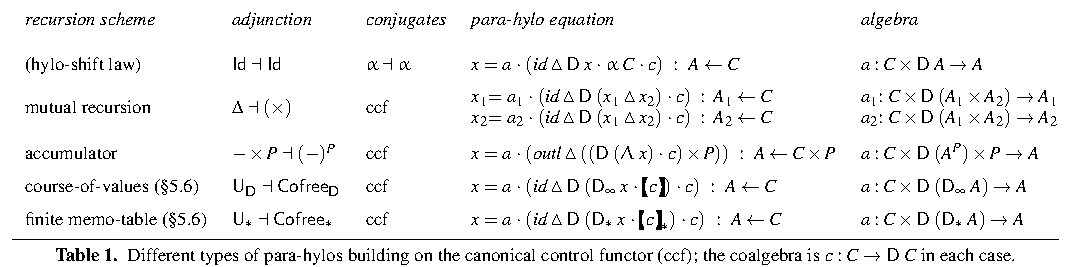
\includegraphics[width = \textwidth, alt = {Table 1 of Hinze, Wu and
        Gibbons: para-hylos built on the canonical control functor, for the
        hylo-shift law, mutual recursion, accumulators, course-of-values
        recursion and finite memo-tables, with their adjunctions,
        conjugates, equations and algebras.}]{types-of-parahylos-crop.pdf}
    \end{sticky}
  \end{center}
  \slideref{R. Hinze, N. Wu, J. Gibbons. \textbf{Conjugate Hylomorphisms, or:
    The Mother of All Structured Recursion Schemes}. POPL 2015.}
  \speakernote{Hinze, Wu and Gibbons: mutual recursion, accumulators,
    course-of-values recursion (dynamic programming) are all hylomorphisms,
    via an adjunction or conjugate pair. Accumulators: curry/uncurry.
    Dynamic programming: the cofree comonad (Part IV). So mechanising
    hylomorphisms covers a lot. Optional slide.}
\end{frame}
